
%%%%%%%%%%%%%%%%%%%%%%%%%%%%%%%%%%%%%%%%%%%%%%%%%%%%%%%%%%%%%%%%%%
\section{Inverter hardware and modulation techniques}
%%%%%%%%%%%%%%%%%%%%%%%%%%%%%%%%%%%%%%%%%%%%%%%%%%%%%%%%%%%%%%%%%%

%%%%%%%%%%%%%%%%%%%%%%%%%%%%%%%%%%%%%%%%%%%%%%%%%%%%%%%%%%%%%%%%%%
\subsection{Two-level voltage source inverter}
%%%%%%%%%%%%%%%%%%%%%%%%%%%%%%%%%%%%%%%%%%%%%%%%%%%%%%%%%%%%%%%%%%

%%%%%%%%%%%%%%%%%%%%%%%%%%%%%%%%%%%%%%%%%%%%%%%%%%%%%%%%%%%%%
%% Two-level voltage source inverter (2L-VSI) %%
%%%%%%%%%%%%%%%%%%%%%%%%%%%%%%%%%%%%%%%%%%%%%%%%%%%%%%%%%%%%%
\begin{frame}
    \frametitle{Two-level voltage source inverter (2L-VSI)}
    \begin{figure}
        \begin{circuitikz}
            \draw (0,0) node[cute spdt up arrow, xscale=-1] (Sw1) {};
            \draw (1.5,-1.5) node[cute spdt down arrow, xscale=-1] (Sw2) {};
            \draw (3,-3) node[cute spdt down arrow, xscale=-1] (Sw3) {};
            \draw (Sw2.in) to [short, -o] ++(4,0) coordinate (out2);
            \draw (Sw1.in) to [short] ++(3.75,0) to [short, -o] (Sw1.in -| out2) coordinate (out1);
            \draw (Sw3.in) to [short, i=$i_{\mathrm{c}}(t)$] ($(Sw3.in |- Sw3.in)!0.5!(Sw3.in -| out2)$) to [short, -o] (Sw3.in -| out2) coordinate (out3);
            \draw (Sw3.in |- Sw2.in) to [short, i=$i_{\mathrm{b}}(t)$] ($(Sw3.in |- Sw2.in)!0.5!(Sw2.in -| out2)$) to [short, -o] (Sw2.in -| out2);
            \draw (Sw3.in |- Sw1.in) to [short, i=$i_{\mathrm{a}}(t)$] ($(Sw3.in |- Sw1.in)!0.5!(Sw1.in -| out2)$) to [short, -o] (Sw1.in -| out2);
            \draw (out1) to [open, v^=$u_{\mathrm{a\text{-}b}}(t)$, voltage = straight] (out2);
            \draw (out2) to [open, v^=$u_{\mathrm{b\text{-}c}}(t)$, voltage = straight] (out3);
            \draw ($(out3) + (1.5,0)$) to [open, v_=$u_{\mathrm{c\text{-}a}}(t)$, voltage = straight] ($(out1) + (1.5,0)$);
            \draw (Sw1-out 1.n) to [short, -*] ++(0,0.5) coordinate (int1);
            \draw (Sw3-out 2.s) to [short] ++(0,-0.5) coordinate (int3);
            \draw (int3) to [short] (int3 -| Sw1-out 2.s) coordinate (int4) to [short, *-] (Sw1-out 2.s);
            \draw node[crossingshape, name=x1, rotate=-90] at (out1 -| Sw2-out 1.n) {};
            \draw (x1.west) to [short] (int1 -| x1.west) coordinate (int2) to [short] (int1);
            \draw (x1.east) to [short] (Sw2-out 1.n);
            \draw (int1) to [short] ++(-1,0) to [short, i_<=$i_\mathrm{dc}(t)$, -o] ++(-1,0) coordinate (in1);
            \draw (int4) to [short, -o] ++(-2,0) coordinate (in2);
            \draw (in1) to [open, v=$\frac{u_\mathrm{dc}(t)}{2}$, voltage = straight] ($(in2)!0.5!(in1)$) coordinate (mid);
            \draw (mid) to [open, v=$\frac{u_\mathrm{dc}(t)}{2}$, voltage = straight] (in2);
            \draw (mid) node[rground, rotate=-90, name = gnd1]{};
            \draw node[anchor = east, xshift=-0.3cm] at (Sw1) {$s_1(t)$};
            \draw node[anchor = east, xshift=-0.3cm] at (Sw2) {$s_2(t)$};
            \draw node[anchor = east, xshift=-0.3cm] at (Sw3) {$s_3(t)$};
            \draw (Sw2-out 2.s) to [short, -*] (int3 -| Sw2-out 2.s);
            \draw node[crossingshape, name=x2, rotate=-90] at (out1 -| Sw3-out 1.n) {};
            \draw node[crossingshape, name=x3, rotate=-90] at (out2 -| Sw3-out 1.n) {};
            \draw (x3.west) to [short] (x2.east);
            \draw (x3.east) to [short] (Sw3-out 1.n);
            \draw (x2.west) to [short] (int2 -| x2.west) to [short,-*] (int2);
            \draw ($(out2  |- in2) + (-0.5,0)$) node[rground, anchor = north, name = gnd2]{};
            \draw[->] ($(out3) + (0,-0.2)$) to ($(out3 |- gnd2) + (0,0.2)$);
            \draw[->] ($(out2) + (-0.5,-0.2)$) to ($(out2 |- gnd2) + (-0.5,0.2)$);
            \draw[->] ($(out1) + (-1,-0.2)$) to ($(out1 |- gnd2) + (-1,0.2)$);
            \draw ($(out3)!0.5!(gnd2) + (0.5,0)$) node[anchor = west] {$u_{\mathrm{ai/bi/ci}}(t)$};
        \end{circuitikz}
        \caption{Idealized switch representation of a three-phase two-level inverter (note that the reference voltage potential is typically only a virtual point and physically not present in the circuit).}
        \label{fig:idealized_switch_three_phase_bridge_converter}
    \end{figure}
\end{frame}

%%%%%%%%%%%%%%%%%%%%%%%%%%%%%%%%%%%%%%%%%%%%%%%%%%%%%%%%%%%%%
%% Circuit realization %%
%%%%%%%%%%%%%%%%%%%%%%%%%%%%%%%%%%%%%%%%%%%%%%%%%%%%%%%%%%%%%
\begin{frame}
    \frametitle{2L-VSI: circuit realization}
    \begin{figure}
        \begin{circuitikz}[]
            \draw (0,4) coordinate (A) to [capacitor, *-*, v = $\frac{u_\mathrm{dc}(t)}{2}$, voltage = straight] ++(0,-3) coordinate (Z) to [capacitor, *-*, v = $\frac{u_\mathrm{dc}(t)}{2}$, voltage = straight] ++(0,-3) coordinate (B)
            (Z) node[rground, rotate=-90, name = gnd1]{}
            (A) to [short, *-o] ++(-2,0) coordinate (Y)
            (B) to [short, *-o] ++(-2,0) coordinate (X)
            (Y) to [open, o-o, v = $u_\mathrm{dc}(t)$, voltage = straight] (X)
            (A) to [short, i=$i_\mathrm{dc}(t)$] ++(2,0) coordinate (E)
            to [TLnigbt, n=igbt1, invert, bodydiode] ++(0,-2) coordinate (C)
            to [short, *-] ++(1,0) to [crossing] ++(2,0) to [crossing] ++(2,0)
            to [short, i=$i_{\mathrm{a}}(t)$] ++(1,0) coordinate (U) to [short] ++(1,0) coordinate (G)
            (C) to [short] ++(0,-2)
            to [TLnigbt, n=igbt2, invert, bodydiode] ++(0,-2) coordinate (D)
            (E) to [short, *-] ++(2,0) coordinate (I)
            to [TLnigbt, n=igbt3, invert, bodydiode] ++(0,-2)
            to [short] ++(0,-1) coordinate (F)
            to [short] ++(0,-1)
            to [TLnigbt, n=igbt4, invert, bodydiode] ++(0,-2)
            to [short, -*] ++(-2,0)
            to [short, -o] (B)
            (I) to [short, *-] ++(2,0)
            to [TLnigbt, n=igbt5, invert, bodydiode] ++(0,-2) coordinate (J)
            to [short] ++(0,-2) coordinate (K)
            to [TLnigbt, n=igbt6, invert, bodydiode] ++(0,-2)
            to [short, -*] ++(-2,0)
            (F) to [short, *-] ++(1,0) to [crossing] ++(2,0) to [short, i=$i_{\mathrm{b}}(t)$] ++(1,0) coordinate (V) to [short] ++(1,0) coordinate (H)
            (K) to [short, *-] ++(1,0) to [short, i=$i_{\mathrm{c}}(t)$] ++(1,0) to [short] ++(0.5,0) coordinate(W) to [short] ++(0.5,0) coordinate (L)
            (G) to [open, o-o, v^=$u_{\mathrm{a\text{-}b}}(t)$, voltage = straight] (H)
            (H) to [open, o-o, v^=$u_{\mathrm{b\text{-}c}}(t)$, voltage = straight] (L)
            ($(L) + (1.5,0)$) to [open, v_=$u_{\mathrm{c\text{-}a}}(t)$, voltage = straight] ($(G) + (1.5,0)$);
            \draw let \p1 = (igbt1.B) in node[anchor=south east] at (\x1,\y1) {$T_1$};
            \draw let \p1 = (igbt2.B) in node[anchor=south east] at (\x1,\y1) {$T_2$};
            \draw let \p1 = (igbt3.B) in node[anchor=south east] at (\x1,\y1) {$T_3$};
            \draw let \p1 = (igbt4.B) in node[anchor=south east] at (\x1,\y1) {$T_4$};
            \draw let \p1 = (igbt5.B) in node[anchor=south east] at (\x1,\y1) {$T_5$};
            \draw let \p1 = (igbt6.B) in node[anchor=south east] at (\x1,\y1) {$T_6$};
            \draw
            (W |- D) node[rground, anchor = south, name = gnd2]{};
            \draw[->] ($(W) + (0.5,-0.2)$) to ($(W |- gnd2) + (0.5,0.2)$);
            \draw[->] ($(V) + (0.5,-0.2)$) to ($(V |- gnd2) + (0.5,0.2)$);
            \draw[->] ($(U) + (0,-0.2)$) to ($(U |- gnd2) + (0,0.2)$);
            \draw ($(W)!0.5!(gnd2) + (0.5,0)$) node[anchor = west] {$u_{\mathrm{ai/bi/ci}}(t)$};
        \end{circuitikz}
        \caption{2L-VSI realization with insulated gate bipolar transistors (IGBTs) and anti-parallel diodes.}
        \label{fig:2L-VSI_IGBT}
    \end{figure}
\end{frame}

%%%%%%%%%%%%%%%%%%%%%%%%%%%%%%%%%%%%%%%%%%%%%%%%%%%%%%%%%%%%%
%% Circuit realization (cont.) %%
%%%%%%%%%%%%%%%%%%%%%%%%%%%%%%%%%%%%%%%%%%%%%%%%%%%%%%%%%%%%%
\begin{frame}
    \frametitle{2L-VSI: circuit realization (cont.)}
    \vspace{-0.2cm}
    \begin{figure}
        \begin{circuitikz}[]
            \draw (0,4) coordinate (A) to [capacitor, *-*, v = $\frac{u_\mathrm{dc}(t)}{2}$, voltage = straight] ++(0,-3) coordinate (Z) to [capacitor, *-*, v = $\frac{u_\mathrm{dc}(t)}{2}$, voltage = straight] ++(0,-3) coordinate (B)
            (Z) node[rground, rotate=-90, name = gnd1]{}
            (A) to [short, *-o] ++(-2,0) coordinate (Y)
            (B) to [short, *-o] ++(-2,0) coordinate (X)
            (Y) to [open, o-o, v = $u_\mathrm{dc}(t)$, voltage = straight] (X)
            (A) to [short, i=$i_\mathrm{dc}(t)$] ++(2,0) coordinate (E)
            to [Tnigfete, n=mosfet1, invert, bodydiode] ++(0,-2) coordinate (C)
            to [short, *-] ++(1,0) to [crossing] ++(2,0) to [crossing] ++(2,0)
            to [short, i=$i_{\mathrm{a}}(t)$] ++(1,0) coordinate (U) to [short] ++(1,0) coordinate (G)
            (C) to [short] ++(0,-2)
            to [Tnigfete, n=mosfet2, invert, bodydiode] ++(0,-2) coordinate (D)
            (E) to [short, *-] ++(2,0) coordinate (I)
            to [Tnigfete, n=mosfet3, invert, bodydiode] ++(0,-2)
            to [short] ++(0,-1) coordinate (F)
            to [short] ++(0,-1)
            to [Tnigfete, n=mosfet4, invert, bodydiode] ++(0,-2)
            to [short, -*] ++(-2,0)
            to [short, -o] (B)
            (I) to [short, *-] ++(2,0)
            to [Tnigfete, n=mosfet5, invert, bodydiode] ++(0,-2) coordinate (J)
            to [short] ++(0,-2) coordinate (K)
            to [Tnigfete, n=mosfet6, invert, bodydiode] ++(0,-2)
            to [short, -*] ++(-2,0)
            (F) to [short, *-] ++(1,0) to [crossing] ++(2,0) to [short, i=$i_{\mathrm{b}}(t)$] ++(1,0) coordinate (V) to [short] ++(1,0) coordinate (H)
            (K) to [short, *-] ++(1,0) to [short, i=$i_{\mathrm{c}}(t)$] ++(1,0) to [short] ++(0.5,0) coordinate(W) to [short] ++(0.5,0) coordinate (L)
            (G) to [open, o-o, v^=$u_{\mathrm{a\text{-}b}}(t)$, voltage = straight] (H)
            (H) to [open, o-o, v^=$u_{\mathrm{b\text{-}c}}(t)$, voltage = straight] (L)
            ($(L) + (1.5,0)$) to [open, v_=$u_{\mathrm{c\text{-}a}}(t)$, voltage = straight] ($(G) + (1.5,0)$);
            \draw let \p1 = (mosfet1.G) in node[anchor=south] at (\x1,\y1) {$T_1$};
            \draw let \p1 = (mosfet2.G) in node[anchor=south] at (\x1,\y1) {$T_2$};
            \draw let \p1 = (mosfet3.G) in node[anchor=south] at (\x1,\y1) {$T_3$};
            \draw let \p1 = (mosfet4.G) in node[anchor=south] at (\x1,\y1) {$T_4$};
            \draw let \p1 = (mosfet5.G) in node[anchor=south] at (\x1,\y1) {$T_5$};
            \draw let \p1 = (mosfet6.G) in node[anchor=south] at (\x1,\y1) {$T_6$};
            \draw
            (W |- D) node[rground, anchor = south, name = gnd2]{};
            \draw[->] ($(W) + (0.5,-0.2)$) to ($(W |- gnd2) + (0.5,0.2)$);
            \draw[->] ($(V) + (0.5,-0.2)$) to ($(V |- gnd2) + (0.5,0.2)$);
            \draw[->] ($(U) + (0,-0.2)$) to ($(U |- gnd2) + (0,0.2)$);
            \draw ($(W)!0.5!(gnd2) + (0.5,0)$) node[anchor = west] {$u_{\mathrm{ai/bi/ci}}(t)$};
        \end{circuitikz}
        \caption{2L-VSI realization with metal-oxide-semiconductor field-effect transistors (MOSFETs) and anti-parallel diodes.}
        \label{fig:2L-VSI_MOSFET}
    \end{figure}
\end{frame}


%%%%%%%%%%%%%%%%%%%%%%%%%%%%%%%%%%%%%%%%%%%%%%%%%%%%%%%%%%%%%
%% Typical power semiconductor devices for three-phase inverters %%
%%%%%%%%%%%%%%%%%%%%%%%%%%%%%%%%%%%%%%%%%%%%%%%%%%%%%%%%%%%%%
\begin{frame}
    \frametitle{Typical power semiconductor devices for three-phase inverters}
    \begin{table}
        \centering

        \small
        \setlength{\tabcolsep}{4pt}
        \renewcommand{\arraystretch}{1.15}
        \begin{tabular}{p{2.2cm} p{3cm} p{3cm} p{2.2cm} p{3.5cm}}
            \toprule
            Technology                                                                                                                                                                                                                                                                                & Voltage rating & Current ratings & Switching freq. & Apparent power range \\
            \midrule
            \href{https://en.wikipedia.org/wiki/Power_MOSFET}{Si MOSFET}                                                                                                                                                                                                                              &
            Typ.: \SIrange{20}{600}{\volt}                                                                                                                                                                                                                             \newline Max: \SI{1600}{\volt} &
            Typ.: \SIrange{1}{200}{\ampere}\newline Max: \SI{350}{\ampere}                                                                                                                                                                                                                            &
            \SIrange{20}{100}{\kilo\hertz}                                                                                                                                                                                                                                                            &
            Typ.: \SIrange{0.1}{50}{\kilo\volt\ampere}                                                                                                                                                                                                                                                                                                                            \\
            \href{https://en.wikipedia.org/wiki/Insulated-gate_bipolar_transistor}{IGBT}                                                                                                                                                                                                              &
            Typ.: \SIrange{650}{1700}{\volt}\newline Max: \SI{6500}{\volt}                                                                                                                                                                                                                            &
            Typ.: \SIrange{35}{1400}{\ampere}\newline Max: \SI{4000}{\ampere}                                                                                                                                                                                                                         &
            \SIrange{2}{50}{\kilo\hertz}                                                                                                                                                                                                                                                              &
            Typ.: \SIrange{1}{5000}{\kilo\volt\ampere}                                                                                                                                                                                                                                                                                                                            \\
            \href{https://en.wikipedia.org/wiki/Gate_turn-off_thyristor}{GTO}                                                                                                                                                                                                                         &
            Typ.: \SIrange{1350}{4500}{\volt}\newline Max: \SI{6000}{\volt}                                                                                                                                                                                                                           &
            Typ.: \SIrange{600}{4000}{\ampere}\newline Max: \SI{6000}{\ampere}                                                                                                                                                                                                                        &
            \SIrange{0.2}{0.5}{\kilo\hertz}                                                                                                                                                                                                                                                           &
            Typ.: \SIrange{1}{20}{\mega\volt\ampere}                                                                                                                                                                                                                                                                                                                              \\
            \href{https://en.wikipedia.org/wiki/Integrated_gate-commutated_thyristor}{IGCT}                                                                                                                                                                                                           &
            Typ.: \SIrange{4500}{6000}{\volt}\newline Max: \SI{6500}{\volt}                                                                                                                                                                                                                           &
            Typ.: \SIrange{1000}{2700}{\ampere}\newline Max: \SI{6000}{\ampere}                                                                                                                                                                                                                       &
            \SIrange{0.5}{1}{\kilo\hertz}                                                                                                                                                                                                                                                             &
            Typ.: \SIrange{0.1}{30}{\mega\volt\ampere}                                                                                                                                                                                                                                                                                                                            \\
            \href{https://en.wikipedia.org/wiki/Silicon_carbide\#Power_electronic_devices}{SiC MOSFET}                                                                                                                                                                                                &
            Typ.: \SIrange{650}{1700}{\volt}\newline Max: \SI{3300}{\volt}                                                                                                                                                                                                                            &
            Typ.: \SIrange{75}{1000}{\ampere}\newline Max: \SI{1200}{\ampere}                                                                                                                                                                                                                         &
            \SIrange{20}{200}{\kilo\hertz}                                                                                                                                                                                                                                                            &
            Typ.: \SIrange{1}{1000}{\kilo\volt\ampere}                                                                                                                                                                                                                                                                                                                            \\
            \href{https://en.wikipedia.org/wiki/Gallium_nitride\#Transistors_and_power_ICs}{GaN HEMT}                                                                                                                                                                                                 &
            Typ.: \SIrange{60}{650}{\volt}\newline Max: \SI{1250}{\volt}                                                                                                                                                                                                                              &
            Typ.:\SIrange{1}{100}{\ampere}\newline Max: \SI{300}{\ampere}                                                                                                                                                                                                                             &
            \SIrange{40}{100}{\kilo\hertz}                                                                                                                                                                                                                                                            &
            Typ.: \SIrange{0.5}{15}{\kilo\volt\ampere}                                                                                                                                                                                                                                                                                                                            \\
            \bottomrule
        \end{tabular}
        \caption{Comparison of commercially used power semiconductor technologies for three-phase inverters.}
    \end{table}
\end{frame}

%%%%%%%%%%%%%%%%%%%%%%%%%%%%%%%%%%%%%%%%%%%%%%%%%%%%%%%%%%%%%
%% Switching function and phase voltages %%
%%%%%%%%%%%%%%%%%%%%%%%%%%%%%%%%%%%%%%%%%%%%%%%%%%%%%%%%%%%%%
\begin{frame}
    \frametitle{Switching function and phase voltages}
    Per VSI lag we define a \hl{switching function}
    \begin{equation}
        \begin{split}
            s_\mathrm{a}(t) & = \begin{cases}
                                    1,  & \text{if } T_1 \text{ is on and } T_2 \text{ is off}, \\
                                    -1, & \text{if } T_1 \text{ is off and } T_2 \text{ is on},
                                \end{cases} \\
            s_\mathrm{b}(t) & = \begin{cases}
                                    1,  & \text{if } T_3 \text{ is on and } T_4 \text{ is off}, \\
                                    -1, & \text{if } T_3 \text{ is off and } T_4 \text{ is on},
                                \end{cases} \\
            s_\mathrm{c}(t) & = \begin{cases}
                                    1,  & \text{if } T_5 \text{ is on and } T_6 \text{ is off}, \\
                                    -1, & \text{if } T_5 \text{ is off and } T_6 \text{ is on}.
                                \end{cases}
        \end{split}
        \label{eq:2L_VSI_switching_functions}
    \end{equation}
    From this we receive the \hl{VSI phase voltages} (with lower index $\mathrm{i}$ for inverter output) against reference as
    \begin{equation}
        u_\mathrm{ai}(t) = \frac{u_\mathrm{dc}(t)}{2} s_\mathrm{a}(t), \quad
        u_\mathrm{bi}(t) = \frac{u_\mathrm{dc}(t)}{2} s_\mathrm{b}(t), \quad
        u_\mathrm{ci}(t) = \frac{u_\mathrm{dc}(t)}{2} s_\mathrm{c}(t)
        \label{eq:VSI_phase_voltages}
    \end{equation}
    and the \hl{DC-link current} is $i_\mathrm{dc}(t) = \sum_{k=\mathrm{a, b, c}}s_k(t)i_k(t)$.
\end{frame}

%%%%%%%%%%%%%%%%%%%%%%%%%%%%%%%%%%%%%%%%%%%%%%%%%%%%%%%%%%%%%
%% Three-phase converter with symmetric load in star connection %%
%%%%%%%%%%%%%%%%%%%%%%%%%%%%%%%%%%%%%%%%%%%%%%%%%%%%%%%%%%%%%
\begin{frame}
    \frametitle{Three-phase converter with symmetric load in star connection}
    \vspace{-0.3cm}
    \begin{figure}
        \begin{circuitikz}[]
            \draw (0,4) coordinate (A) to [capacitor, *-*, v = $\frac{u_\mathrm{dc}(t)}{2}$, voltage = straight] ++(0,-3) coordinate (Z) to [capacitor, *-*, v = $\frac{u_\mathrm{dc}(t)}{2}$, voltage = straight] ++(0,-3) coordinate (B)
            (Z) node[rground, rotate=-90, name = gnd1]{}
            (A) to [short, *-o] ++(-2,0) coordinate (Y)
            (B) to [short, *-o] ++(-2,0) coordinate (X)
            (Y) to [open, o-o, v = $u_\mathrm{dc}(t)$, voltage = straight] (X)
            (A) to [short, i=$i_{\mathrm{dc}}(t)$] ++(2,0) coordinate (E)
            to [TLnigbt, n=igbt1, invert, bodydiode] ++(0,-2) coordinate (C)
            to [short, *-] ++(1,0) to [crossing] ++(2,0) to [crossing] ++(2,0)
            to [short, i=$i_{\mathrm{a}}(t)$] ++(1,0) coordinate (U) to [short] ++(1,0) coordinate (G)
            (C) to [short] ++(0,-2)
            to [TLnigbt, n=igbt2, invert, bodydiode] ++(0,-2) coordinate (D)
            (E) to [short, *-] ++(2,0) coordinate (I)
            to [TLnigbt, n=igbt3, invert, bodydiode] ++(0,-2)
            to [short] ++(0,-1) coordinate (F)
            to [short] ++(0,-1)
            to [TLnigbt, n=igbt4, invert, bodydiode] ++(0,-2)
            to [short, -*] ++(-2,0)
            to [short, -o] (B)
            (I) to [short, *-] ++(2,0)
            to [TLnigbt, n=igbt5, invert, bodydiode] ++(0,-2) coordinate (J)
            to [short] ++(0,-2) coordinate (K)
            to [TLnigbt, n=igbt6, invert, bodydiode] ++(0,-2)
            to [short, -*] ++(-2,0)
            (F) to [short, *-] ++(1,0) to [crossing] ++(2,0) to [short, i=$i_{\mathrm{b}}(t)$] ++(1,0) coordinate (V) to [short] ++(1,0) coordinate (H)
            (K) to [short, *-] ++(1,0) to [short, i=$i_{\mathrm{c}}(t)$] ++(1,0) to [short] ++(0.5,0) coordinate(W) to [short] ++(0.5,0) coordinate (L);
            \draw (H) to [inductor, v^=$u_{\mathrm{b}}(t)$, voltage=straight] ++(1.5,0) to [short,-*] ++(1,0) coordinate (N)
            (L) to [inductor, v^=$u_{\mathrm{c}}(t)$, voltage=straight] ++(1.5,0) to [short] (\tikztostart) -| (N)
            (G) to [inductor, v^=$u_{\mathrm{a}}(t)$, voltage=straight] ++(1.5,0) to [short] (\tikztostart) -| (N);
            \draw let \p1 = (igbt1.B) in node[anchor=south east] at (\x1,\y1) {$T_1$};
            \draw let \p1 = (igbt2.B) in node[anchor=south east] at (\x1,\y1) {$T_2$};
            \draw let \p1 = (igbt3.B) in node[anchor=south east] at (\x1,\y1) {$T_3$};
            \draw let \p1 = (igbt4.B) in node[anchor=south east] at (\x1,\y1) {$T_4$};
            \draw let \p1 = (igbt5.B) in node[anchor=south east] at (\x1,\y1) {$T_5$};
            \draw let \p1 = (igbt6.B) in node[anchor=south east] at (\x1,\y1) {$T_6$};
            \draw (W |- D) node[rground, anchor = south, name = gnd2]{};
            \draw[->] ($(W) + (0.5,-0.2)$) to ($(W |- gnd2) + (0.5,0.2)$);
            \draw[->] ($(V) + (0.5,-0.2)$) to ($(V |- gnd2) + (0.5,0.2)$);
            \draw[->] ($(U) + (0,-0.2)$) to ($(U |- gnd2) + (0,0.2)$);
            \draw ($(W)!0.5!(gnd2) + (0.5,0)$) node[anchor = west] {$u_{\mathrm{ai/bi/ci}}(t)$};
            \draw[->] ($(N) + (0,-1.25)$) to ($(N |- gnd2) + (0,0.2)$);
            \draw (N |- D) node[rground, anchor = south, name = gnd3]{};
            \draw ($(W)!0.5!(gnd3)+ (1.5,0)$) node[anchor = west] {$u_{\mathrm{N}}(t)$};
            \draw (N) node[anchor = west] {$\mathrm{N}$};
        \end{circuitikz}
        \caption{Three-phase VSI with symmetric load in star connection}
        \label{fig:VSI_three_phase_two_level_bridge_converter_load_star}
    \end{figure}
\end{frame}

%%%%%%%%%%%%%%%%%%%%%%%%%%%%%%%%%%%%%%%%%%%%%%%%%%%%%%%%%%%%%
%% Three-phase converter with symmetric load in star connection (cont.) %%
%%%%%%%%%%%%%%%%%%%%%%%%%%%%%%%%%%%%%%%%%%%%%%%%%%%%%%%%%%%%%
\begin{frame}
    \frametitle{Three-phase converter with symmetric load in star connection (cont.)}
    Assuming a \hl{star-connected load} and that the star point is not connected to ground, $u_{\mathrm{N}}(t)\neq 0$ may occur leading to a load voltage of
    \begin{equation}
        u_{\mathrm{a}}(t) = u_{\mathrm{ai}}(t) - u_{\mathrm{N}}(t), \quad u_{\mathrm{b}}(t) = u_{\mathrm{bi}}(t) - u_{\mathrm{N}}(t), \quad u_{\mathrm{c}}(t) = u_{\mathrm{ci}}(t) - u_{\mathrm{N}}(t).
    \end{equation}\pause
    To calculate $u_{\mathrm{N}}(t)$ one can utilize the load equation (assuming an \hl{inductive load} as approximation of an electrical machine):
    \begin{equation}
        u_{i}(t) = L \frac{\mathrm{d}}{\mathrm{d}t} i_{i}(t) + u_{\mathrm{N}}(t), \quad i\in \{\mathrm{a, b, c}\}
    \end{equation}\pause
    summing up to
    \begin{equation}
        3u_{\mathrm{N}}(t) +  L \frac{\mathrm{d}}{\mathrm{d}t} \underbrace{\left(i_{\mathrm{a}}(t) + i_{\mathrm{b}}(t) + i_{\mathrm{c}}(t)\right)}_{=0} = u_{\mathrm{ai}}(t) + u_{\mathrm{bi}}(t) +u_{\mathrm{ci}}(t)
    \end{equation}\pause
    and finally delivering the \hl{star-to-ground voltage} as
    \begin{equation}
        u_{\mathrm{N}}(t) = \frac{1}{3} \left(u_{\mathrm{ai}}(t) + u_{\mathrm{bi}}(t) +u_{\mathrm{ci}}(t)\right).
    \end{equation}
\end{frame}

%%%%%%%%%%%%%%%%%%%%%%%%%%%%%%%%%%%%%%%%%%%%%%%%%%%%%%%%%%%%%
%% Three-phase converter with symmetric load in star connection (cont.) %%
%%%%%%%%%%%%%%%%%%%%%%%%%%%%%%%%%%%%%%%%%%%%%%%%%%%%%%%%%%%%%
\begin{frame}[b]
    \frametitle{Three-phase converter with symmetric load in star connection (cont.)}
    \vspace{1em}
    \begin{table}
        \renewcommand{\arraystretch}{1.25}
        \centering
        \begin{tabular}{c c c c c c c c c c c c c c}
            \toprule
            $\mathrm{No.}$ & $s_\mathrm{a}$ & $s_\mathrm{b}$ & $s_\mathrm{c}$ & $\frac{u_{\mathrm{ai}}}{u_\mathrm{dc}}$ & $\frac{u_{\mathrm{bi}}}{u_\mathrm{dc}}$ & $\frac{u_{\mathrm{ci}}}{u_\mathrm{dc}}$ & $\frac{u_{\mathrm{a}}}{u_\mathrm{dc}}$ & $\frac{u_{\mathrm{b}}}{u_\mathrm{dc}}$ & $\frac{u_{\mathrm{c}}}{u_\mathrm{dc}}$ & $\frac{u_{\mathrm{a\text{-}b}}}{u_\mathrm{dc}}$ & $\frac{u_{\mathrm{b\text{-}c}}}{u_\mathrm{dc}}$ & $\frac{u_{\mathrm{c\text{-}a}}}{u_\mathrm{dc}}$ & $\frac{u_{\mathrm{N}}}{u_\mathrm{dc}}$ \\
            \midrule
            $0$            & $-1$           & $-1$           & $-1$           & $-\frac{1}{2}$                          & $-\frac{1}{2}$                          & $-\frac{1}{2}$                          & $0$                                    & $0$                                    & $0$                                    & $0$                                             & $0$                                             & $0$                                             & $-\frac{1}{2}$                         \\

            $1$            & $+1$           & $-1$           & $-1$           & $+\frac{1}{2}$                          & $-\frac{1}{2}$                          & $-\frac{1}{2}$                          & $+\frac{2}{3}$                         & $-\frac{1}{3}$                         & $-\frac{1}{3}$                         & $+1$                                            & $0$                                             & $-1$                                            & $-\frac{1}{6}$                         \\

            $2$            & $+1$           & $+1$           & $-1$           & $+\frac{1}{2}$                          & $+\frac{1}{2}$                          & $-\frac{1}{2}$                          & $+\frac{1}{3}$                         & $+\frac{1}{3}$                         & $-\frac{2}{3}$                         & $0$                                             & $+1$                                            & $-1$                                            & $+\frac{1}{6}$                         \\

            $3$            & $-1$           & $+1$           & $-1$           & $-\frac{1}{2}$                          & $+\frac{1}{2}$                          & $-\frac{1}{2}$                          & $-\frac{1}{3}$                         & $+\frac{2}{3}$                         & $-\frac{1}{3}$                         & $-1$                                            & $+1$                                            & $0$                                             & $-\frac{1}{6}$                         \\

            $4$            & $-1$           & $+1$           & $+1$           & $-\frac{1}{2}$                          & $+\frac{1}{2}$                          & $+\frac{1}{2}$                          & $-\frac{2}{3}$                         & $+\frac{1}{3}$                         & $+\frac{1}{3}$                         & $-1$                                            & $0$                                             & $+1$                                            & $+\frac{1}{6}$                         \\

            $5$            & $-1$           & $-1$           & $+1$           & $-\frac{1}{2}$                          & $-\frac{1}{2}$                          & $+\frac{1}{2}$                          & $-\frac{1}{3}$                         & $-\frac{1}{3}$                         & $+\frac{2}{3}$                         & $0$                                             & $-1$                                            & $1$                                             & $-\frac{1}{6}$                         \\

            $6$            & $+1$           & $-1$           & $+1$           & $+\frac{1}{2}$                          & $-\frac{1}{2}$                          & $+\frac{1}{2}$                          & $+\frac{1}{3}$                         & $-\frac{2}{3}$                         & $+\frac{1}{3}$                         & $1$                                             & $-1$                                            & $0$                                             & $+\frac{1}{6}$                         \\

            $7$            & $+1$           & $+1$           & $+1$           & $+\frac{1}{2}$                          & $+\frac{1}{2}$                          & $+\frac{1}{2}$                          & $0$                                    & $0$                                    & $0$                                    & $0$                                             & $0$                                             & $0$                                             & $+\frac{1}{2}$                         \\

            \bottomrule
        \end{tabular}
        \caption{Switching states and resulting voltages of the three-phase 2L-VSI with symmetric load in star connection (with $2^3=8$ possible switching states)}
        \label{tab:VSI_three_phase_two_level_bridge_converter_load_star}
    \end{table}
\end{frame}

%%%%%%%%%%%%%%%%%%%%%%%%%%%%%%%%%%%%%%%%%%%%%%%%%%%%%%%%%%%%%
%% Elementary voltage vectors %%
%%%%%%%%%%%%%%%%%%%%%%%%%%%%%%%%%%%%%%%%%%%%%%%%%%%%%%%%%%%%%
\begin{frame}
    \frametitle{Elementary voltage vectors}
    Based on \eqref{eq:2L_VSI_switching_functions} and \eqref{eq:VSI_phase_voltages} we define the \hl{elementary voltage vectors} as
    \begin{equation}
        \bm{u}_\mathrm{i}(t) = \frac{u_\mathrm{dc}(t)}{2} \begin{bmatrix}
            s_\mathrm{a}(t) \\
            s_\mathrm{b}(t) \\
            s_\mathrm{c}(t)
        \end{bmatrix}\in \left\{\bm{u}_{\mathrm{i}0}(t), \bm{u}_{\mathrm{i}1}(t), \ldots, \bm{u}_{\mathrm{i}7}(t) \right\}.
    \end{equation}
    Given the discrete nature of the switching functions, \hl{only $2^3=8$ different voltage vectors} can be generated by the three-phase 2L-VSI  with $\bm{u}_{\mathrm{i}k}(t)$ being the voltage vector corresponding to the switching state $k$ as defined in \tabref{tab:VSI_three_phase_two_level_bridge_converter_load_star}.\pause  Applying the \hl{simplified Clarke transformation} \eqref{eq:Clarke_transformation_zero_component_free} to the elementary voltage vectors, we can represent them in the $\upalpha\upbeta$-plane:
    \begin{equation}
        \bm{u}_\mathrm{\upalpha\upbeta i}(t) = \begin{bmatrix}
            u_\mathrm{\upalpha i}(t) \\
            u_\mathrm{\upbeta i}(t)
        \end{bmatrix}= \bm{T}_{23}\bm{u}_\mathrm{i}(t).
    \end{equation}
    Here, we \hl{neglect the voltage zero-component} as the star connection condition \eqref{eq:star_connection_conditions} prevents the generation of a zero-component current (not considering \hl{parasitic effects}, cf. \figref{fig:VSI_three_phase_two_level_bridge_converter_load_star_parasitic_currents}).
\end{frame}

%%%%%%%%%%%%%%%%%%%%%%%%%%%%%%%%%%%%%%%%%%%%%%%%%%%%%%%%%%%%%
%% Elementary voltage vectors in the $\upalpha\upbeta$-plane %%
%%%%%%%%%%%%%%%%%%%%%%%%%%%%%%%%%%%%%%%%%%%%%%%%%%%%%%%%%%%%%
\begin{frame}[b]
    \frametitle{Elementary voltage vectors in the $\upalpha\upbeta$-plane}
    \vspace{0.3em}
    \begin{columns}[T,onlytextwidth]
        \begin{column}{0.52\textwidth}
            \begin{table}
                \setlength{\tabcolsep}{4pt}
                \renewcommand{\arraystretch}{1.2}
                \centering
                \begin{tabular}{c c c c c c}
                    \toprule
                    $\mathrm{No.}$ & $s_\mathrm{a}$ & $s_\mathrm{b}$ & $s_\mathrm{c}$ & $\frac{u_{\mathrm{\upalpha i}}}{u_\mathrm{dc}}$ & $\frac{u_{\mathrm{\upbeta i}}}{u_\mathrm{dc}}$ \\
                    \midrule
                    $0$            & $-1$           & $-1$           & $-1$           & $0$                                             & $0$                                            \\
                    $1$            & $+1$           & $-1$           & $-1$           & $+\frac{2}{3}$                                  & $0$                                            \\
                    $2$            & $+1$           & $+1$           & $-1$           & $+\frac{1}{3}$                                  & $+\frac{1}{\sqrt{3}}$                          \\
                    $3$            & $-1$           & $+1$           & $-1$           & $-\frac{1}{3}$                                  & $+\frac{1}{\sqrt{3}}$                          \\
                    $4$            & $-1$           & $+1$           & $+1$           & $-\frac{2}{3}$                                  & $0$                                            \\
                    $5$            & $-1$           & $-1$           & $+1$           & $-\frac{1}{3}$                                  & $-\frac{1}{\sqrt{3}}$                          \\
                    $6$            & $+1$           & $-1$           & $+1$           & $+\frac{1}{3}$                                  & $-\frac{1}{\sqrt{3}}$                          \\
                    $7$            & $+1$           & $+1$           & $+1$           & $0$                                             & $0$                                            \\
                    \bottomrule
                \end{tabular}
                \caption{Switching states and normalized elementary voltage vectors of the three-phase 2L-VSI.}
                \label{tab:VSI_three_phase_two_level_bridge_converter_load_star}
            \end{table}
        \end{column}
        \begin{column}{0.47\textwidth}
            \centering
            \vspace{-0.275cm}
            \begin{figure}
                \begin{tikzpicture}[x=1.25cm,y=1.25cm,>=Latex]
                    \coordinate (u0) at (0,0);
                    \coordinate (u1) at (2,0);
                    \coordinate (u2) at (1,1.732);
                    \coordinate (u3) at (-1,1.732);
                    \coordinate (u4) at (-2,0);
                    \coordinate (u5) at (-1,-1.732);
                    \coordinate (u6) at (1,-1.732);
                    \coordinate (betaMax) at ($(u2)!0.5!(u3)$);

                    \draw[->,thin] (-2.5,0) -- (2.7,0) node[below] {$u_{\upalpha i}$};
                    \draw[->,thin] (0,-2.2) -- (0,2.2) node[left] {$u_{\upbeta i}$};
                    \draw[gray!70,thick] (u1) -- (u2) -- (u3) -- (u4) -- (u5) -- (u6) -- cycle;

                    \draw[thin] (u1) ++(0,0.08) -- ++(0,-0.16);
                    \draw[thin] ($(u1) + (0.03,-0.15)$) -- ++(0.1,-0.28) node[below right] {$\frac{2}{3}u_\mathrm{dc}$};

                    \draw[thin] (betaMax) ++(0.08,0.08) -- ++(0.35,0.2) node[above right] {$\frac{1}{\sqrt{3}}u_\mathrm{dc}$};
                    \draw[thin] (betaMax) ++(0.08,0) -- ++(-0.16,0);

                    \draw[signalalpha,->,thick] (u0) -- (u1);
                    \draw[signalalpha,->,thick] (u0) -- (u2);
                    \draw[signalalpha,->,thick] (u0) -- (u3);
                    \draw[signalalpha,->,thick] (u0) -- (u4);
                    \draw[signalalpha,->,thick] (u0) -- (u5);
                    \draw[signalalpha,->,thick] (u0) -- (u6);

                    \node[above right] at (u1) {$\bm{u}_{\mathrm{i}1}$};
                    \node[above right] at (u2) {$\bm{u}_{\mathrm{i}2}$};
                    \node[above left] at (u3) {$\bm{u}_{\mathrm{i}3}$};
                    \node[above left] at (u4) {$\bm{u}_{\mathrm{i}4}$};
                    \node[below left] at (u5) {$\bm{u}_{\mathrm{i}5}$};
                    \node[below right] at (u6) {$\bm{u}_{\mathrm{i}6}$};

                    \fill[signalalpha] (u0) circle (3pt);
                    \node[below right, xshift=0.08cm] at (u0) {$\bm{u}_{\mathrm{i}7}$};
                    \node[above right, xshift=0.08cm] at (u0) {$\bm{u}_{\mathrm{i}0}$};
                \end{tikzpicture}
                \caption{Elementary voltage vectors in the $\alpha\beta$ plane.}
                \label{fig:elementary_voltages_alpha_beta}
            \end{figure}
        \end{column}
    \end{columns}
\end{frame}




%%%%%%%%%%%%%%%%%%%%%%%%%%%%%%%%%%%%%%%%%%%%%%%%%%%%%%%%%%%%%
%% Three-phase converter with symmetric load in star connection %%
%%%%%%%%%%%%%%%%%%%%%%%%%%%%%%%%%%%%%%%%%%%%%%%%%%%%%%%%%%%%%
\begin{frame}
    \frametitle{Parasitic common mode currents}

    \begin{figure}
        \begin{circuitikz}[scale=0.8, every node/.style={scale=0.8}]
            \draw (0,4) coordinate (A) to [capacitor, *-*, v = $\frac{u_\mathrm{dc}(t)}{2}$, voltage = straight] ++(0,-3) coordinate (Z) to [capacitor, *-*, v = $\frac{u_\mathrm{dc}(t)}{2}$, voltage = straight] ++(0,-3) coordinate (B)
            (Z) node[rground, rotate=-90, name = gnd1]{}
            (A) to [short, *-] ++(-2,0) coordinate (Y)
            (B) to [short, *-] ++(-2,0) coordinate (X)
            (Y) to [open, o-o, v = $u_\mathrm{dc}(t)$, voltage = straight] (X)
            (A) to [short, i_>=$i_{\mathrm{dc}}(t)$] ++(2,0) coordinate (E)
            to [TLnigbt, n=igbt1, invert, bodydiode] ++(0,-2) coordinate (C)
            to [short, *-] ++(1,0) to [crossing] ++(2,0) to [crossing] ++(2,0)
            to [short, i=$i_{\mathrm{a}}(t)$] ++(1,0) coordinate (U) to [short] ++(1,0) coordinate (G)
            (C) to [short] ++(0,-2)
            to [TLnigbt, n=igbt2, invert, bodydiode] ++(0,-2) coordinate (D)
            (E) to [short, *-] ++(2,0) coordinate (I)
            to [TLnigbt, n=igbt3, invert, bodydiode] ++(0,-2)
            to [short] ++(0,-1) coordinate (F)
            to [short] ++(0,-1)
            to [TLnigbt, n=igbt4, invert, bodydiode] ++(0,-2)
            to [short, -*] ++(-2,0)
            to [short] (B)
            (I) to [short, *-] ++(2,0)
            to [TLnigbt, n=igbt5, invert, bodydiode] ++(0,-2) coordinate (J)
            to [short] ++(0,-2) coordinate (K)
            to [TLnigbt, n=igbt6, invert, bodydiode] ++(0,-2) coordinate (T6low)
            to [short, -*] ++(-2,0)
            (F) to [short, *-] ++(1,0) to [crossing] ++(2,0) to [short, i=$i_{\mathrm{b}}(t)$] ++(1,0) coordinate (V) to [short] ++(1,0) coordinate (H)
            (K) to [short, *-] ++(1,0) to [short, i=$i_{\mathrm{c}}(t)$] ++(1,0) to [short] ++(0.5,0) coordinate(W) to [short] ++(0.5,0) coordinate (L);
            \draw (H) to [inductor, v^=$u_{\mathrm{b}}(t)$, voltage=straight] ++(1.5,0) to [short,-*] ++(1,0) coordinate (N)
            (L) to [inductor, v^=$u_{\mathrm{c}}(t)$, voltage=straight] ++(1.5,0) to [short] (\tikztostart) -| (N)
            (G) to [inductor, v^=$u_{\mathrm{a}}(t)$, voltage=straight] ++(1.5,0) to [short] (\tikztostart) -| (N);
            \draw let \p1 = (igbt1.B) in node[anchor=south east] at (\x1,\y1) {$T_1$};
            \draw let \p1 = (igbt2.B) in node[anchor=south east] at (\x1,\y1) {$T_2$};
            \draw let \p1 = (igbt3.B) in node[anchor=south east] at (\x1,\y1) {$T_3$};
            \draw let \p1 = (igbt4.B) in node[anchor=south east] at (\x1,\y1) {$T_4$};
            \draw let \p1 = (igbt5.B) in node[anchor=south east] at (\x1,\y1) {$T_5$};
            \draw let \p1 = (igbt6.B) in node[anchor=south east] at (\x1,\y1) {$T_6$};
            \draw (W |- D) node[rground, anchor = south, name = gnd2]{};
            \draw[->] ($(W) + (0.5,-0.2)$) to ($(W |- gnd2) + (0.5,0.2)$);
            \draw[->] ($(V) + (0.5,-0.2)$) to ($(V |- gnd2) + (0.5,0.2)$);
            \draw[->] ($(U) + (0,-0.2)$) to ($(U |- gnd2) + (0,0.2)$);
            \draw ($(W)!0.5!(gnd2) + (0.5,0)$) node[anchor = west] {$u_{\mathrm{ai/bi/ci}}(t)$};
            \draw[->] ($(N) + (0,-1.25)$) to ($(N |- gnd2) + (0,0.2)$);
            \draw (N |- D) node[rground, anchor = south, name = gnd3]{};
            \draw ($(W)!0.5!(gnd3)+ (1.5,0)$) node[anchor = west] {$u_{\mathrm{N}}(t)$};
            \draw (N) node[anchor = south west] {$\mathrm{N}$};

            %rectangular box below (X) -> upper left corner of the box and to (T6low) -> upper right corner of the box. add 2 vertical space distance
            \draw[dashed] (B) to [capacitor] ++(0,-1.25);
            \coordinate (housingSW) at ($(X) + (0,-2.0)$);
            \coordinate (housingNE) at ($(T6low) + (0,-1.25)$);
            \coordinate (housingSE) at (housingSW -| housingNE);
            \coordinate (housingEast) at ($(housingSE)!0.5!(housingNE)$);
            \draw[dashed] (housingSW) rectangle (housingNE) node[ pos=0.5] (housing) {VSI housing};
            \draw[dashed] (N) to [capacitor] ++(2,0) coordinate (housingLinkStart) to [short, i=$i_{\mathrm{CM}}(t)$] (\tikztostart |- housingEast) to [short] (housingEast);
            \coordinate (housingLinkBend) at (housingLinkStart |- housingEast);
            \draw (housingLinkBend) to [short,*-] ++(0,-0.0) node[rground, anchor = north, name = gnd4]{};

        \end{circuitikz}
        \caption{Common-mode current $i_{\mathrm{CM}}(t)$ due to $u_{\mathrm{N}}(t)\neq 0$ and capacitive parasitic coupling of the VSI and machine via ground (note: further parasitic current paths exist, e.g., via the bearing and rotor).}
        \label{fig:VSI_three_phase_two_level_bridge_converter_load_star_parasitic_currents}
    \end{figure}
\end{frame}

%%%%%%%%%%%%%%%%%%%%%%%%%%%%%%%%%%%%%%%%%%%%%%%%%%%%%%%%%%%%%
%% Inverter induced bearing currents %%
%%%%%%%%%%%%%%%%%%%%%%%%%%%%%%%%%%%%%%%%%%%%%%%%%%%%%%%%%%%%%
\begin{frame}
    \frametitle{Inverter induced bearing currents}
    \vspace{-0.2cm}
    \begin{figure}
        \centering
        \begin{subfigure}[b]{0.58\textwidth}
            \centering
            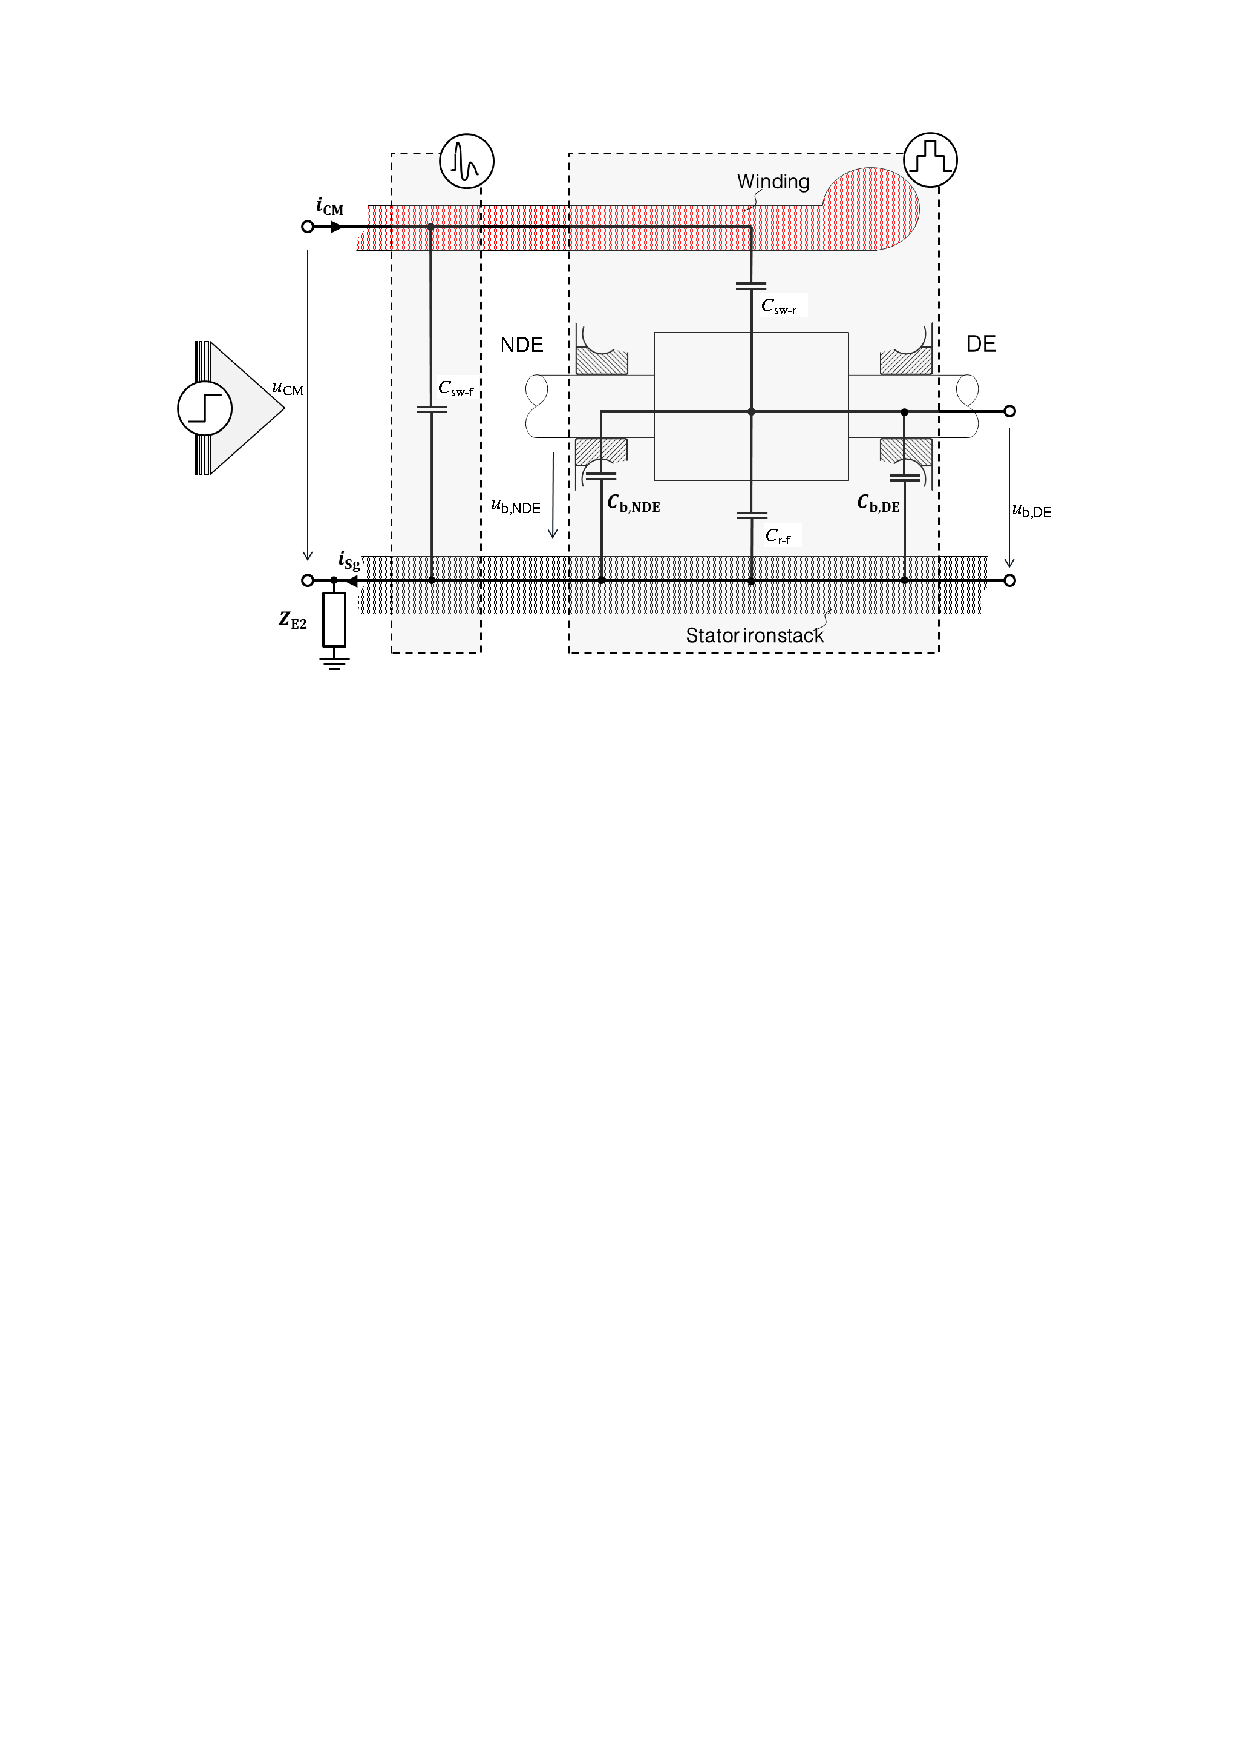
\includegraphics[width=\linewidth,height=0.65\textheight,keepaspectratio]{fig/lec02/Equivalent_capactive circuit.pdf}
            \caption{Equivalent capacitive circuit of the parasitic coupling paths.}
        \end{subfigure}
        \hfill
        \begin{subfigure}[b]{0.41\textwidth}
            \centering
            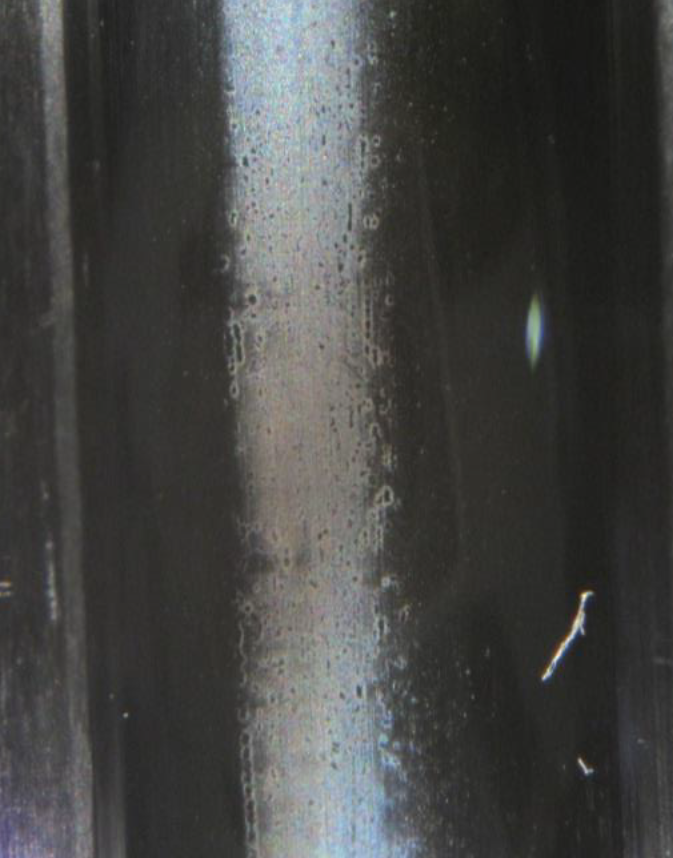
\includegraphics[width=\linewidth,height=0.65\textheight,keepaspectratio]{fig/lec02/Damaged_bearing.png}
            \caption{Bearing surface damage.}
        \end{subfigure}
        \caption{Inverter-induced bearing currents can lead to electrical discharge machining damage at the bearing surfaces (source: \href{https://tuprints.ulb.tu-darmstadt.de/id/eprint/19393}{TU Darmstadt}, \href{https://creativecommons.org/licenses/by/4.0/deed.en}{CC BY 4.0}).}
        \label{fig:inverter_induced_bearing_currents}
    \end{figure}
\end{frame}

%%%%%%%%%%%%%%%%%%%%%%%%%%%%%%%%%%%%%%%%%%%%%%%%%%%%%%%%%%%%%%%%%%
\subsection{Pulse width modulation}
%%%%%%%%%%%%%%%%%%%%%%%%%%%%%%%%%%%%%%%%%%%%%%%%%%%%%%%%%%%%%%%%%%